\chapter{Từ trường của dòng điện chạy trong dây dẫn thẳng dài}
\section{Lý thuyết trọng tâm}
\subsection{Đường sức từ tạo bởi dòng điện qua dây thẳng dài}
Là những đường tròn đồng tâm nằm trong  mặt phẳng vuông góc với dây dẫn và có tâm là giao điểm của mặt phẳng và dây dẫn. 
\begin{center}
	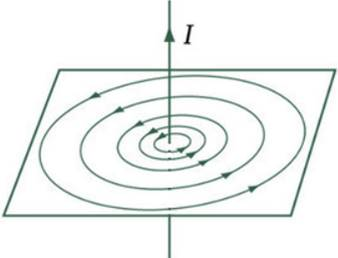
\includegraphics[scale=0.8]{../figs/VN11-PH-26-L-018-1-h106.jpg}
\end{center}
\subsection{Véctơ cảm ứng từ $\vec{B}$ do dòng điện thẳng dài gây ra}

\begin{center}
	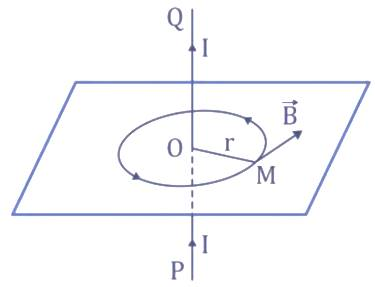
\includegraphics[scale=0.8]{../figs/VN11-PH-26-L-018-1-h83.jpg}
\end{center}
\begin{itemize}
	\item Điểm đặt: tại điểm đang xét.
	\item Phương: vuông góc với mặt phẳng chứa dây dẫn và điểm ta xét.
	\item Chiều: xác định theo quy tắc nắm tay phải: để bàn tay phải sao cho ngón cái nằm dọc theo dây dẫn và chỉ theo chiều dòng điện, khi đó các ngón kia khum lại cho ta chiều của các đường sức từ.
	\item Độ lớn:  
	\begin{equation}
	B=2\cdot 10^{-7}\dfrac{I}{r},
	\end{equation}
	trong đó,
	\begin{itemize}
		\item $I$ là cường độ của dòng điện, đơn vị ampère (A). 
		\item $r$ là khoảng cách từ điểm ta xét tới dòng điện, đơn vị mét (m).
		\item $B$ là cảm ứng từ, đơn vị tesla (T).
	\end{itemize}

\end{itemize}

\subsection{Nguyên lý chồng chất từ trường}
 Véctơ cảm ứng từ tại một điểm do nhiều dòng điện gây ra bằng tổng các véctơ cảm ứng từ do từng dòng điện gây ra tại điểm đó.
\begin{equation}
\vec{B}=\vec{B}_1+\vec{B}_2+\vec{B}_3+...+\vec{B}_\text{n},
\end{equation} 
trong đó, $\vec{B}_1, \ \vec{B}_2, \ \vec{B}_3,..., \ \vec{B}_\text{n}$ là cảm ứng từ do các dòng điện $I_1, \ I_2, \ I_3,..., \ I_\text{n}$ gây ra tại điểm đang xét.

\section{Bài tập}
\begin{dang}{Công thức cảm ứng từ $\vec{B}$ do dòng điện thẳng dài gây ra}
\end{dang}

\textbf{Phương pháp giải}

Áp dụng công thức  $B=2\cdot 10^{-7}\dfrac{I}{r}$, từ đó tìm được giá trị cảm ứng từ $B$, cường độ dòng điện $I$,  khoảng cách $r$ từ điểm ta xét tới dòng điện.

\vspace*{1em}

\vidu{2}	
{Dây dẫn thẳng dài có dòng điện 15 A chạy qua. Cảm ứng từ tại M có độ lớn $2\cdot 10^{-5}\ \text{T}$. Điểm M cách dây một khoảng là
\begin{mcq}(4)
	\item $\text{5}\ \text{cm}$.
	\item $\text{10}\ \text{cm}$.
	\item $\text{15}\ \text{cm}$.
	\item $\text{20}\ \text{cm}$.
\end{mcq}
}
{\begin{center}
	\textbf{Hướng dẫn giải:}
\end{center}

Cảm ứng từ tại những điểm cách dây 10 cm có độ lớn là:

 $B=2\cdot 10^{-7}\dfrac{I}{r}\Rightarrow r=2\cdot 10^{-7}\dfrac{I}{B}=\text{15}\ \text{cm}$.

\textbf{Đáp án: C.}

}

\begin{dang}{Tổng hợp véctơ cảm ứng từ $\vec{B}$ \\bởi nhiều dòng điện thẳng dài gây ra}
\end{dang}

\textbf{Phương pháp giải}
\begin{description}
	
	\item[Bước 1:] Xác định điểm đặt, phương, chiều của véctơ cảm ứng từ $\vec{B}$ do các dòng điện gây ra tại điểm đang xét bằng quy tắc nắm tay phải.
	
	\item[Bước 2:] Sử dụng công thức $B=2\cdot 10^{-7}\dfrac{I}{r}$ để tính cảm ứng từ do các dòng điện thẳng dài gây ra tại điểm đang xét.
	\item[Bước 3:] Áp dụng quy tắc tổng hợp véctơ và nguyên lý chồng chất từ trường để xác định véctơ cảm ứng từ $\vec{B}$ tổng hợp tạo bởi nhiều dòng điện.
	
	\luuy{
	Cảm ứng từ do dòng điện $I_1$, $I_2$ gây ra tại điểm đang xét lần lượt là $\vec{B}_1$, $\vec{B}_2$.
	Cảm ứng từ tổng hợp tại điểm đang xét:
	 \begin{equation}
	 \vec{B}=\vec{B}_1+\vec{B}_2.
	 \end{equation} 
	
Nếu:
\begin{itemize}
	\item $\vec{B}_1$ cùng chiều $\vec{B}_2$ thì độ lớn cảm ứng từ tổng hợp: $B=B_1+B_2$. 
	\item  $\vec{B}_1$ ngược chiều $\vec{B}_2$ thì độ lớn cảm ứng từ tổng hợp: $B=\left| B_1-B_2\right| $. 
	\item $\vec{B}_1$ vuông góc $\vec{B}_2$ thì độ lớn cảm ứng từ tổng hợp: $B=\sqrt{ B_1^2+B_2^2}$.
	\item $\vec{B}_1$ hợp với $\vec{B}_2$ một góc $\alpha$ thì độ lớn cảm ứng từ tổng hợp:
	
	 $B=\sqrt{ B_1^2+B_2^2+2B_1B_2\cos \alpha}$.
\end{itemize}
} 
	
\end{description}
 
\viduii{3}{	
Hai dây dẫn thẳng, rất dài, đặt song song, cách nhau 20 cm trong không khí, có hai dòng điện ngược chiều, có cường độ $I_1=12\ \text{A}$, $I_2=10\ \text{A}$ chạy qua. Xác định cảm ứng từ tổng hợp do hai dòng điện này gây ra tại điểm M cách dây dẫn mang dòng $I_1$   một đoạn 15 cm và cách dây dẫn mang dòng $I_2$ một đoạn 5 cm.

	\begin{mcq}(4)
		\item $\text{2,4}\cdot 10^{-5}\ \text{T}$.
		\item $\text{5,6}\cdot 10^{-5}\ \text{T}$.
		\item $\text{4,6}\cdot 10^{-5}\ \text{T}$.
		\item $\text{3,4}\cdot 10^{-5}\ \text{T}$.
	\end{mcq}}
{\begin{center}
		\textbf{Hướng dẫn giải:}
\end{center}
	\begin{center}
		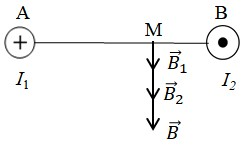
\includegraphics[scale=0.8]{../figs/VN11-PH-26-L-018-1-h84.jpg}
	\end{center}
Giả sử hai dây dẫn đó được đặt vuông góc với mặt phẳng hình vẽ, dòng điện $I_1$  đi vào mặt phẳng giấy tại A, dòng điện $I_2$ đi ra mặt phẳng giấy tại B thì các dòng điện $I_1$   và $I_2$ gây ra tại M các véctơ cảm ứng từ $\vec{B}_1$ và $\vec{B}_2$ có phương chiều như hình vẽ, có độ lớn:

$B_1=2\cdot 10^{-7}\dfrac{I_1}{\text{AM}}=\text{1,6}\cdot 10^{-5}\ \text{T}$, $B_2=2\cdot 10^{-7}\dfrac{I_2}{\text{BM}}=\text{4}\cdot 10^{-5}\ \text{T}$.

Cảm ứng từ tổng hợp tại M là $\vec{B}=\vec{B}_1+\vec{B}_2$.

Vì $\vec{B}_1$ và $\vec{B}_2$ cùng phương, cùng chiều nên $\vec{B}$ cùng phương, cùng chiều với $\vec{B}_1$, $\vec{B}_2$ và có độ lớn $B=B_1+B_2=\text{5,6}\cdot 10^{-5}\ \text{T}$.  

\textbf{	Đáp án: C.}
}

\viduii{3}{	
	Hai dây dẫn thẳng, rất dài, đặt song song, cách nhau 5 cm trong không khí, có hai dòng điện cùng chiều, có cường độ  $I_1=\text{4,5}\ \text{A}$, $I_2=8\ \text{A}$ chạy qua. Xác định độ lớn cảm ứng từ tổng hợp do hai dòng điện này gây ra tại điểm M cách dây dẫn mang dòng $I_1$ 3 cm và cách dây dẫn mang dòng $I_2$  4 cm.

	\begin{mcq}(4)
		\item $ 10^{-5}\ \text{T}$.
		\item $\text{3}\cdot 10^{-5}\ \text{T}$.
		\item $\text{4}\cdot 10^{-5}\ \text{T}$.
		\item $\text{5}\cdot 10^{-5}\ \text{T}$.
	\end{mcq}}{
\begin{center}
		\textbf{Hướng dẫn giải:}
\end{center}
	\begin{center}
		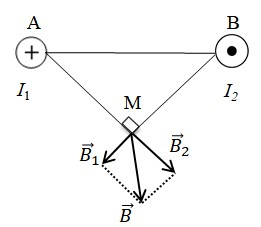
\includegraphics[scale=0.8]{../figs/VN11-PH-26-L-018-1-h85.jpg}
	\end{center}
	
		Giả sử hai dây dẫn được đặt vuông góc với mặt phẳng hình vẽ, dòng điện $I_1$ đi vào tại A, dòng điện $I_2$ đi vào tại B.
	
	Vì $\text{AM}^2+\text{MB}^2=\text{AB}^2$ nên tam giác AMB vuông tại M.
	
	Các dòng điện $I_1$ và $I_2$ gây ra tại M các véctơ cảm ứng từ $\vec{B}_1$ và $\vec{B}_2$ có phương chiều như hình vẽ, có độ lớn:
	
	$B_1=2\cdot 10^{-7}\dfrac{I_1}{\text{AM}}=\text{3}\cdot 10^{-5}\ \text{T}$, $B_2=2\cdot 10^{-7}\dfrac{I_2}{\text{BM}}=\text{4}\cdot 10^{-5}\ \text{T}$.
	
	Cảm ứng từ tổng hợp tại M là: $\vec{B}=\vec{B}_1+\vec{B}_2$.
	
	Vì $\vec{B}_1$ vuông góc với $\vec{B}_2$ nên độ lớn cảm ứng từ tổng hợp $B=\sqrt{ B_1^2+B_2^2}=\text{5}\cdot 10^{-5}\ \text{T}$.  
	
\textbf{	Đáp án: D.}
}


\begin{dang}{Xác định vị trí mà cảm ứng từ tổng hợp $\vec{B}$ bằng 0 hay triệt tiêu}
\end{dang}

\textbf{Phương pháp giải}
\begin{description}
		\item[Bước 1:] Cảm ứng từ tổng hợp bằng 0: $\vec{B}=\vec{B}_1+\vec{B}_2=\vec{0}\Rightarrow \vec{B}_1=-\vec{B}_2 $.
	
	Tức là:
	
		\begin{itemize}
		\item $\vec{B}_1, \ \vec{B}_2$  ngược chiều nhau. 
		\item Độ lớn của chúng bằng nhau: $B_1=B_2$.
		\end{itemize}
	
	\item[Bước 2:] Sử dụng công thức $B=2\cdot 10^{-7}\dfrac{I}{r}$ để tính cảm ứng từ do các dòng điện thẳng dài gây ra tại điểm đang xét.
	
	\item[Bước 3:] Suy ra phương trình chứa các khoảng cách $r_1$ và $r_2$ từ dòng điện $I_1$ và $I_2$ đến điểm đang xét. Kết hợp với đề bài tìm ra $r_1$ và $r_2$ là vị trí để cảm ứng từ tổng hợp tại đó bằng 0.
	
	\luuy{
		\begin{itemize}
			\item Hai dòng điện $I_1$ và $I_2$ \textbf{cùng chiều}: điểm mà cảm ứng từ tổng hợp bằng 0 phải \textbf{phải nằm trên đường thẳng nối A, B; nằm trong đoạn thẳng AB.} và\textbf{ gần dòng điện có cường độ dòng điện nhỏ hơn. }
			\item Hai dòng điện $I_1$ và $I_2$ \textbf{ngược chiều}: điểm mà cảm ứng từ tổng hợp bằng 0 phải \textbf{phải nằm trên đường thẳng nối A, B; nằm ngoài đoạn thẳng AB.} và \textbf{gần dòng điện có cường độ dòng điện nhỏ hơn.}
			\end{itemize}
	} 
	
\end{description}

\viduii{3}{
Hai dây dẫn thẳng, rất dài, đặt song song, cách nhau 15 cm trong không khí, có hai dòng điện cùng chiều, có cường độ $I_1=10\ \text{A}$, $I_2=5\ \text{A}$   chạy qua. Xác định điểm M mà tại đó cảm ứng từ tổng hợp do hai dòng điện này gây ra bằng 0.
	\begin{mcq}
		\item điểm M nằm trên đường thẳng cách dây dẫn mang dòng $I_1$ 10 cm và cách dây dẫn mang dòng $I_2$ 5 cm.	
		\item điểm M nằm trên đường thẳng cách dây dẫn mang dòng $I_1$ 5 cm và cách dây dẫn mang dòng $I_2$ 10 cm.
		\item điểm M nằm trên đường thẳng cách dây dẫn mang dòng $I_1$ $\text{7,5}\ \text{cm}$ và cách dây dẫn mang dòng $I_2$ $\text{7,5}\ \text{cm}$.
		\item điểm M nằm trên đường thẳng cách dây dẫn mang dòng $I_1$ 8 cm và cách dây dẫn mang dòng $I_2$ 7 cm. 
	\end{mcq}}
{\begin{center}
		\textbf{Hướng dẫn giải:}
\end{center}
	\begin{center}
		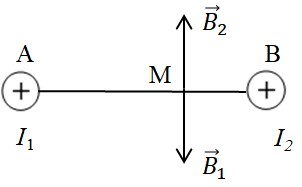
\includegraphics[scale=0.8]{../figs/VN11-PH-26-L-018-1-h86.jpg}
	\end{center}

Giả sử hai dây dẫn được đặt vuông góc với mặt phẳng hình vẽ, dòng $I_1$ đi vào tại A, dòng $I_2$  đi vào tại B. Các dòng điện $I_1$ và $I_2$ gây ra tại M các véctơ cảm ứng từ $\vec{B}_1$ và $\vec{B}_1$.

Để cảm ứng từ tổng hợp tại M bằng 0 thì $\vec{B}=\vec{B}_1+\vec{B}_2=\vec{0}\Rightarrow \vec{B}_1=-\vec{B}_2 $. 


Tức là $\vec{B}_1$ và $\vec{B}_2$ phải cùng phương, ngược chiều và bằng nhau về độ lớn. Để thỏa mãn các điều kiện đó thì M phải nằm trên đường thẳng nối A, B; nằm trong đoạn thẳng AB.

Với $B_1=B_2$ thì ta có:  $2\cdot 10^{-7}\dfrac{I_1}{\text{AM}}=2\cdot 10^{-7}\dfrac{I_2}{\text{BM}}$

$\Leftrightarrow 2\cdot 10^{-7}\dfrac{I_1}{\text{AM}}=2\cdot 10^{-7}\dfrac{I_2}{\text{AB}-\text{AM}}$

$\Rightarrow \text{AM}=\text{10}\ \text{cm}\Rightarrow \text{BM}=\text{5}\ \text{cm}$.

Vậy điểm M phải nằm trên đường thẳng cách dây dẫn mang dòng $I_1$ 10 cm và cách dây dẫn mang dòng $I_2$ 5 cm.

\textbf{	Đáp án: A.}

}
\viduii{3}{	
Hai dây dẫn thẳng, rất dài, đặt song song, cách nhau 12 cm trong không khí, có hai dòng điện ngược chiều, có cường độ $I_1=2\ \text{A}$, $I_2=4\ \text{A}$  chạy qua. Xác định điểm N mà tại đó cảm ứng từ tổng hợp do hai dòng điện này gây ra bằng 0.
	\begin{mcq}
		\item điểm N nằm trên đường thẳng cách dây dẫn mang dòng $I_1$ 18 cm và cách dây dẫn mang dòng $I_2$ 6 cm.	
		\item điểm N nằm trên đường thẳng cách dây dẫn mang dòng $I_1$ 6 cm và cách dây dẫn mang dòng $I_2$ 18 cm.
		\item điểm N nằm trên đường thẳng cách dây dẫn mang dòng $I_1$ $\text{12}\ \text{cm}$ và cách dây dẫn mang dòng $I_2$ $\text{24}\ \text{cm}$.
		\item điểm N nằm trên đường thẳng cách dây dẫn mang dòng $I_1$ 24 cm và cách dây dẫn mang dòng $I_2$ 12 cm. 
	\end{mcq}}
{	\begin{center}
	\textbf{Hướng dẫn giải:}
\end{center}
	\begin{center}
		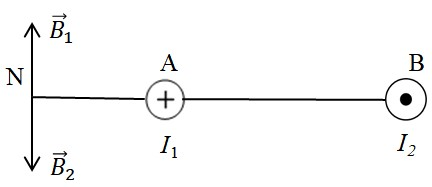
\includegraphics[scale=0.8]{../figs/VN11-PH-26-L-018-1-h87.jpg}
	\end{center}
	
	Giả sử hai dây dẫn được đặt vuông góc với mặt phẳng hình vẽ, dòng $I_1$ đi vào tại A, dòng $I_2$  đi vào tại B. Các dòng điện $I_1$ và $I_2$ gây ra tại N các véctơ cảm ứng từ $\vec{B}_1$ và $\vec{B}_1$.
	
	Để cảm ứng từ tổng hợp tại N bằng 0 thì $\vec{B}=\vec{B}_1+\vec{B}_2=\vec{0}\Rightarrow \vec{B}_1=-\vec{B}_2 $. 
	
	
	Tức là $\vec{B}_1$ và $\vec{B}_2$ phải cùng phương, ngược chiều và bằng nhau về độ lớn. Để thỏa mãn các điều kiện đó thì N phải nằm trên đường thẳng nối A, B; nằm ngoài đoạn thẳng AB.
	
	Với $B_1=B_2$ thì ta có:  $2\cdot 10^{-7}\dfrac{I_1}{\text{AN}}=2\cdot 10^{-7}\dfrac{I_2}{\text{BN}}$
	
	$\Leftrightarrow 2\cdot 10^{-7}\dfrac{I_1}{\text{AN}}=2\cdot 10^{-7}\dfrac{I_2}{\text{AB}+\text{AN}}$
	
	$\Rightarrow \text{AN}=\text{12}\ \text{cm}\Rightarrow \text{BN}=\text{24}\ \text{cm}$.
	
	Vậy điểm N phải nằm trên đường thẳng cách dây dẫn mang dòng $I_1$ 12 cm và cách dây dẫn mang dòng $I_2$ 24 cm.
	
\textbf{	Đáp án: C.}
}	


